
\documentclass[a4paper, 12p]{paper} 
\usepackage[margin=2.5cm]{geometry}
\usepackage{amsmath}
\usepackage{graphicx}
\usepackage{lipsum}
\usepackage{xcolor}
\usepackage{booktabs}
\usepackage{float}
\usepackage{subfigure}
\usepackage{titling}
\usepackage{kotex}
\usepackage{threeparttable}
\usepackage[newfloat]{minted}
\usepackage{caption}
\usepackage{tikz}
\usetikzlibrary{graphs, graphdrawing, automata,positioning}
\usegdlibrary{layered, force}
\usepackage{forest}

\newenvironment{code}{\captionsetup{type=listing}}{}
\SetupFloatingEnvironment{listing}{name=Listing}

\def\code#1{\texttt{#1}}
\sectionfont{\large\sf\bfseries\color{black!70!blue}}
\date{\vspace{-5ex}}
\renewcommand{\familydefault}{\sfdefault}
\renewcommand{\baselinestretch}{1.3} 

\pretitle{\centering\LARGE\bfseries}
\posttitle{\par}
\preauthor{\begin{flushright}\large}
\postauthor{\end{flushright}}

\title{컴파일러 프로젝트 3 결과보고서}
\author{컴퓨터공학과 20171634 박건}
\author{전자공학과 20161453 김규래}

\begin{document} 
\maketitle\hrule{}\bigskip

\begin{center}
\begin{tabular}{ l l }
과목코드 & CSE4120 \\
과목명  & 기초 컴파일러 구성 \\
담당교수 & 정성원 \\
\end{tabular}
\end{center}

\section{개발 목표}
C Language를 간소화한 언어인 C- Language에 대해 Semantic Analysis 를 한 후, Symbol Table을 출력하는 것을 목표로 한다.

\vspace{0.1in}
\noindent\textbf{Symbol Table:} 컴파일 과정에서 identifier 이름과 정보들을 저장해놓는 자료구조이다. 본 과제에서는 Hash table 들의 tree 형태로 심볼테이블을 구현을 하였으며, memory location 과 reference location, 타입 정보를 담는다. 본 과제의 실행 마지막에는, 컴파일한 파일의 심볼 테이블을 출력한다.

\vspace{0.1in}
\noindent\textbf{Semantic Analysis:} Scanning 과 parsing 과정 이후에, 프로그램의 내용, 의미적인 분석을 하는 단계를 말한다. Type checking, 선언후 참조, 함수 선언과 호출의 일치 등을 확인하는 작업이다. Semantic analysis 과정에서 C- 언어의 규칙에 일치하지 않는 구문이 발견될 경우, 에러코드를 출력한다.

\vspace{0.1in}
교재\footnote{Compiler Construction Principles and Practice, K. C. Louden}를 참고하여 \texttt{flex}와 \texttt{bison}을 연동하여 구현한 C- Language의 Parser를 사용하여, Symbol Table을 만들며 Semantic Analysis를 진행하고, 오류가 없을 경우 Symbol Table을 출력한다. 또한 Semantic error가 발생했을 때, 적절한 에러 메시지를 생성하도록 한다.

\section{개요}
본 프로젝트에서는 수업 교재 \textit{Compiler Construction Principles and Practices} 에서 제공하는 파일들을 포함하여 다음과 같은 프로젝트 파일 구성을 갖고 있다. 프로젝트 디렉토리 구성은 Tab.~\ref{table:files} 에 정리돼 있다. 본 프로젝트에서 작성한 파일들은 * 로 표시하였다. 

\begin{table}[H]
  \centering
\begin{threeparttable}
  \caption{프로젝트 파일 구성}\label{table:files}
\begin{tabular}{ll}
  \toprule
파일명 &    내용 \\
        \midrule
  \textbf{globals.h}            & 전역변수 및 타입 정의 \\
  \textbf{main.c}               & 진입점 및 커맨트라인 인자 처리 코드 \\
  \textbf{util.h, util.c}       & 프로젝트에서 사용되는 유틸리티 코드 \\
  \textbf{scan.h, scan.c}       & AST 노드 구조체, AST 생성 관련 코드 \\
  \textbf{lex.l}                & Flex 의 lexing 규칙 정의 \\
  \textbf{parser.y}             & Bison 의 parsing 파싱 규칙 정의 \\
  \textbf{*analyze.h, *analyze.c} & Semantic Analysis 관련 코드 \\
  \textbf{*symtab.h, *symtab.c}   & Symbol Table 생성 관련 코드 \\
 \bottomrule
\end{tabular}
\end{threeparttable}\\
\end{table}

\begin{figure}[H]
\tikz\graph[layered layout]
{
"\texttt{lex.l}" -> [densely dashed] {"\texttt{lex.yy.c}", "\texttt{lex.yy.h}"},
"\texttt{parser.y}" -> [densely dashed] {"\texttt{parser.tab.c}", "\texttt{parser.tab.h}"},
"\texttt{globals.h}" -> {"\texttt{util.h}", "\texttt{lex.l}", "\texttt{parser.y}", "\texttt{main.c}", "\texttt{analyze.c}"},
"\texttt{lex.yy.h}" -> {"\texttt{parser.y}", "\texttt{util.c}",  "\texttt{main.c}"},
"\texttt{util.h}" -> {"\texttt{main.c}", "\texttt{util.c}"},
"\texttt{scan.h}" -> {"\texttt{scan.c}", "\texttt{globals.h}", "\texttt{lex.l}", "\texttt{main.c}", "\texttt{parser.y}", "\texttt{scan.c}", "\texttt{util.h}", "\texttt{analyze.h}"},
"\texttt{parser.tab.h}" -> {"\texttt{globals.h}"},
"\texttt{analyze.h}" -> {"\texttt{analyze.c}", "\texttt{main.c}"},
"\texttt{symtab.h}" -> {"\texttt{symtab.c}", "\texttt{analyze.h}", "\texttt{main.c}"},
};
\caption{프로젝트 파일 종속 관계}\label{fig:dep}
\end{figure}

프로젝트의 디펜던시 그래프는 Fig.~\ref{fig:dep} 과 같다. 프로젝트의 역할 분담 현황은 Tab.~\ref{table:slave} 에 정리하였다.

\begin{table}[H]
  \centering
\begin{threeparttable}
  \caption{구성원 역할 분담}\label{table:slave}
\begin{tabular}{cl}
  \toprule
구성원 &  열할 \\
        \midrule
  \textbf{김규래}  & 심볼테이블을 \code{symtab.c, symtab.h}에 작성. 테스트 파일, 커버리지 리포트 스크립트 작성 \\
  \textbf{박건}   & 진입점 및 커맨트라인 인자 처리 코드, semantic analysis 를 \code{analyze.h, analyze.c} 에 작성 \\
 \bottomrule
\end{tabular}
\end{threeparttable}\\
\end{table}

\subsection{사용방법}
구현물의 사용방법은 지시사항대로, \code{project\_3} 에 16조의 조 번호를 prefix 로 붙인 것이다. \code{--latex} 를 입력할 경우 AST 의 \LaTeX 코드 덤프를 출력한다.

\begin{minted}[frame=lines,
      framesep=2mm,
      baselinestretch=0.5]{sh}
$ make
$ ./project3_16 <file>
$ ./project3_16
Usage: ./project3_16 [--ast] [--latex] <source> [<source2> ...]
\end{minted}

\section{개발내용}
여기서부터는 개발한 내용에 관한 구체적인 묘사를 하겠다.

\subsection{Symbol Table}

\begin{figure}[ht]
  \centering
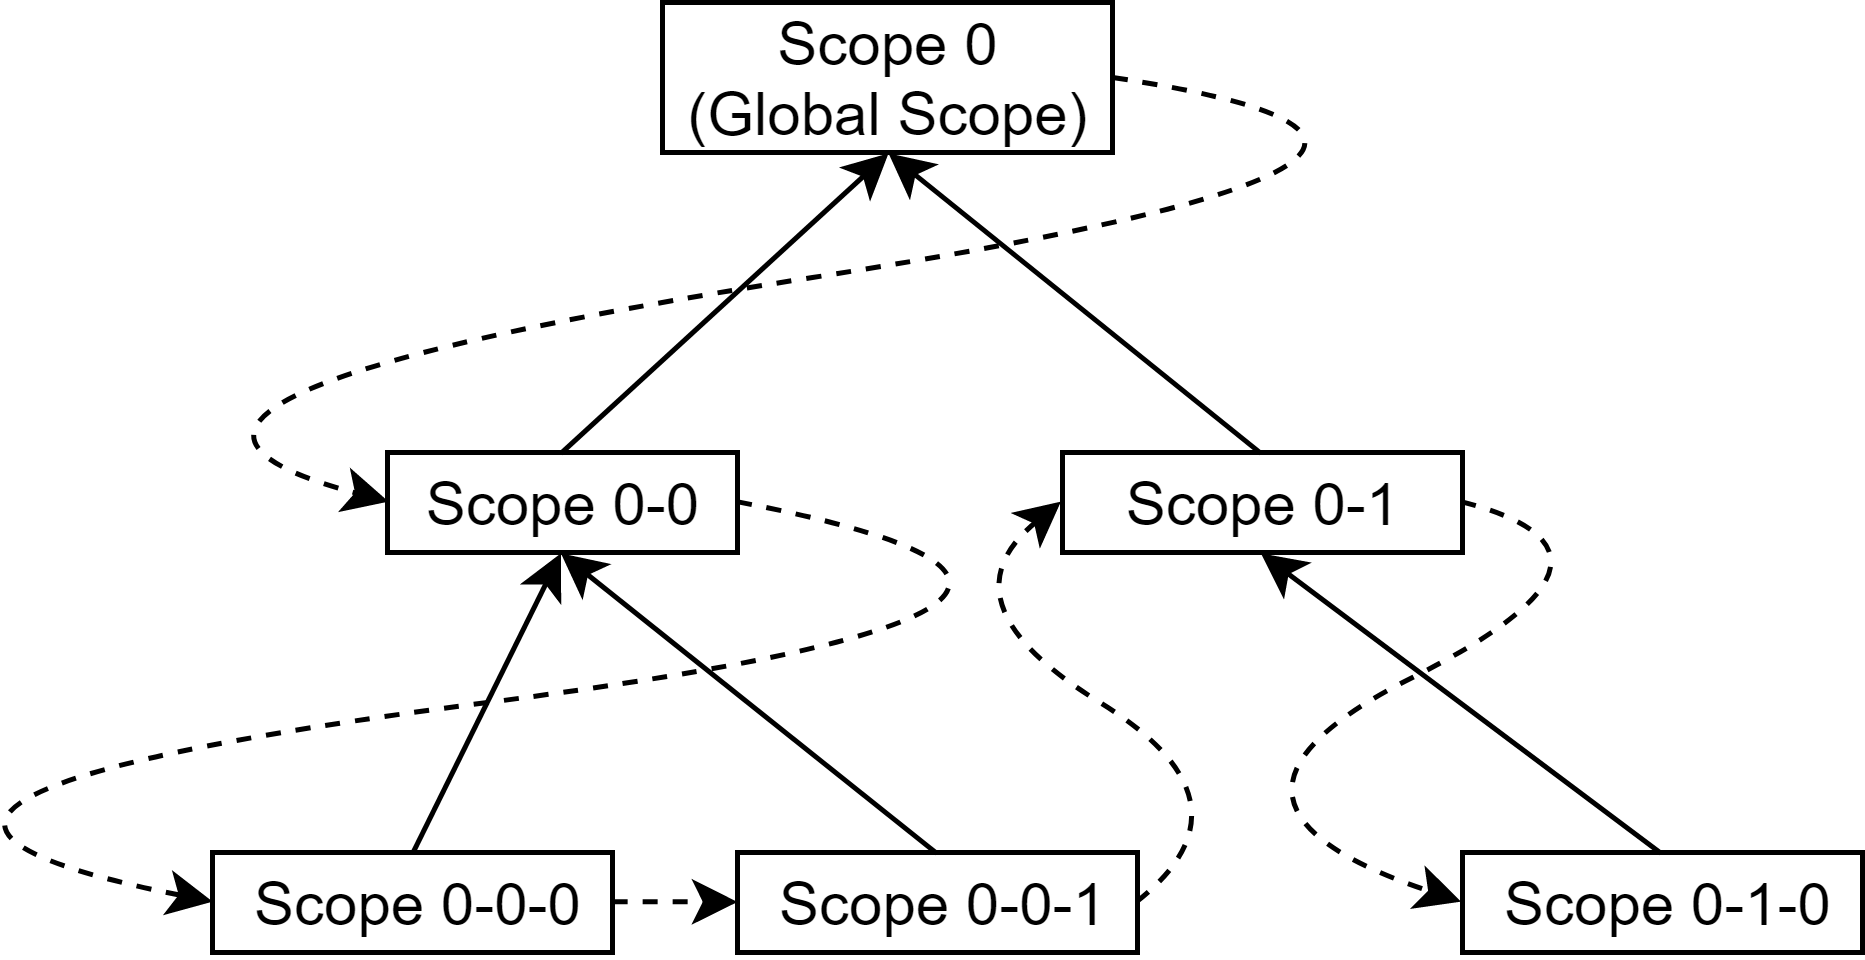
\includegraphics[scale=0.15]{figs/symtabtree.png}
\caption{Symbol Table Tree 의 구조.}\label{fig:symtabtree}
\end{figure}

먼저, 심볼 테이블의 구현을 설명하겠다. 심볼 테이블은 기본적으로 각 스코프당 하나씩 생성이 되도록 하였고, 각 스코프는 상위 스코프를 가리키도록 해서 tree 를 이루도록 했다. Symbol table dump 를 출력하기 위해서 tree 의 모든 노드들은 생성 순서대로 linked list 로 접근할 수도 있다. 이러한 심블 테이블의 구조는 Fig.~\ref{fig:symtabtree} 에 시각화돼있다.

Symbol table tree 의 각 노드들은 scope 가 하나 추가될 때마다 상위 스코프의 child node 로 생성이 되며, 아래의 소스코드와 같은 인터페이스로 구현하였다. 기존에 semantic analysis 를 진행하던 scope 를 벗어날 경우, 현재 가리키고 있는 symbol table node 는 parent 로 변경된다.

\begin{minted}[frame=lines,
      framesep=2mm,
      baselinestretch=0.5]{c}
/* 심볼 테이블 초기화 */
SymTable st_init(void (*freeRecord)(Record));

/* 심볼 테이블에 심볼과 심볼에 대한 정보를 추가 */
void st_insert(SymTable state, 
              const char* name,
              Record record);

/* 새로운 스코프에 들어갈 경우 Scope tree 에 노드를 추가 */
void st_enter_scope(SymTable state);

/* 기존 스코프를 벗어날 경우 parent scope node 로 이동 */
void st_exit_scope(SymTable state); 

/* 심볼 테이블에서 심볼 정보를 검색 (없을 경우 NULL 반환) */
Record st_lookup(SymTable state, char* name); 

/* 심볼 테이블의 메모리를 해제 */
void st_free(SymTable state); 

/* 심볼 테이블 출력 */
void printSymTab(SymTable state, const char* heading, void (*print)(const char*, Record)) 
\end{minted}

Symbol table lookup 의 경우에는, 상위 스코프에 symbol 이 존재하는 것만을 체크하면 되기 때문에, tree 의 node 들은 parent 들만 가리키는 것으로 충분하다.

\begin{minted}[frame=lines,
      framesep=2mm,
      baselinestretch=0.5]{c}
struct ActivationRecord {
    int loc, scope;
    enum SymbolType kind;
    enum TypeKind type;
    enum VPFType vpf;

    union {
        struct {
            int num_params;
            enum SymbolType* param_types;
        } func;
        int arr_size;
    };

    // list of referenced line numbers
    int num_linenos;
    int* linenos;
};
\end{minted}

심볼테이블의 각 symbol 의 정보를 담는 entry 는 위와 같이 구현하였다. 각 symbol record 는 symbol 의 타입과 런타임 메모리 위치, 선언 위치, 그리고 참조 위치를 담는다. 배열의 경우에는 배열 길이 또한 담게 하였다. 함수의 경우에는 argument 의 갯수와 타입, 리턴 값의 타입을 저장한다.

\subsection{Semantic Analysis}

Semantic analysis 는 AST 를 차례대로 순회하며 타입, 인자의 갯수, 선언 여부 같은 것들을 체크한다. 자세한 사항은 명세에 나와있으므로 생략한다. Type checking 은 name equivalence 로 하였고, 아래는 AST 순회 과정에서 각 노드의 synthesized attribute 를 기록 및 전파하기 위해서 추가로 구현한 구조체이다. 

\begin{minted}[frame=lines,
      framesep=2mm,
      baselinestretch=0.5]{c}
enum SymbolType {
    SymUnknown,
    SymVariable,
    SymArray,
    SymFunction,
};

struct NodeRec {
    // Omitted
    union {
        struct {
            enum SymbolType kind;
        };
    } attr;
    // Omitted
};
\end{minted}

Semantic analysis 는 2-pass 가 아닌 1-pass 로 하였다. 그러므로 scope 관련된 체크들을 하는 동시에 type 에 관한 체크를 진행한다.

\noindent\textbf{Variable Shadowing:} 이 구현체에서는 variable shadowing 을 허락하는 것으로 하고, 가장 가까운 상위 스코프의 symbol 을 참조하도록 하였다.

\section{분석내용}
\subsection{Test Case}\label{case}
프로그램의 정확성을 실험하기 위해 다음과 같은 테스트 파일을 만들어 테스트하였고, 이 외에 메뉴얼에서 제시하는 semantic rule 각각에 대하여 test code 를 하나씩 작성하였다. 그리고 \code{Julia} 언어로 된 스크립트를 통해서 한번에 test coverage 를 출력해서 작업을 진행하였다.

아래는 사용한 테스트 케이스 중 하나이다.
\begin{minted}[frame=lines,
      framesep=2mm,
      baselinestretch=0.5]{c}
int arr[10];
int brr[20];

void f(void) {
    ;
}

int func(int parA[], int parB) {
    int a[10];
    int i;
    i = 0;
    while (parB == 0) {
        int wvar;
        parA[i] = parB * func(parA, i) * (parA[i] + parA[i+1]/parB);
        parB = parB - 1;
        i = i + 1;
        if(parB = parA[12])
            if (wvar == 1)
                i = 0;
        else i = 1;
    }

    return parA[2];
}

int crr[30];

void main(void) {
    int tmp;

    while (tmp = 1) {
        int one;
        one = arr[1];
        if (one == brr[2])
            tmp = one == brr[3];
        else {
            int two;
            int tmp;

            two = arr[2];
            while(arr[one] == brr[tmp]) {
                int tmp;
                if (1) {
                    int tmp;
                    tmp = one;
                }
            }
            tmp = two;
        }
    }
    tmp = func(arr, 45);
}
\end{minted}


\subsection{Error Code}
\begin{figure}[H]
  \centering
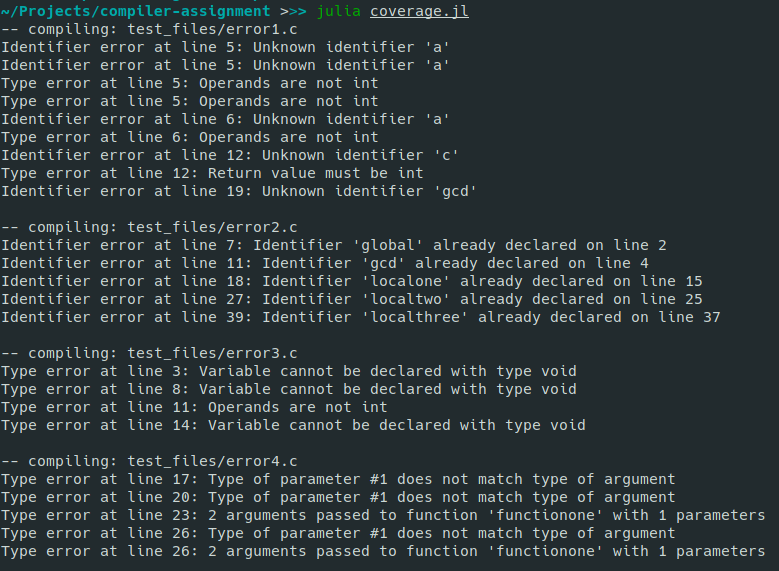
\includegraphics[scale=0.5]{figs/coverage.png}
\caption{Semantic Analysis 의 Test Coverage.}\label{fig:coverage}
\end{figure}

Julia 스크립트를 이용해서 semantic error 구현의 test coverage 를 출력하는 모습을 Fig.~\ref{fig:coverage} 에서 볼 수 있다. 각 파일별로 주입한 에러의 목록이 있으며, 출력한 test coverage 의 내용과 대조를 해가면서 작업을 하였다. Fig.~\ref{fig:coverage} 에서는,

\begin{itemize}
\item 선업되지 않은 식별자
\item 식별자 중복 선언
\item void 타입 식별자 선언
\item 함수 인자 타입 일치
\end{itemize}

를 파일 순서대로 체크해서 에러 코드를 출력하는 모습을 볼 수 있다.

\begin{figure}[H]
  \centering
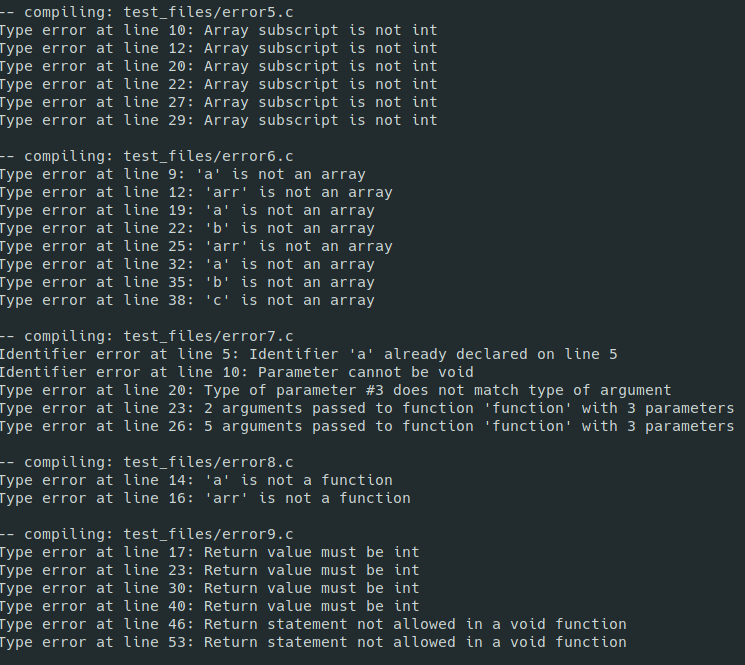
\includegraphics[scale=0.5]{figs/coverage2.png}
\caption{Semantic Analysis 의 Test Coverage.}\label{fig:coverage2}
\end{figure}

Fig.~\ref{fig:coverage2} 에서는

\begin{itemize}
\item Array subscript 타입의 int 여부
\item Array Subscript가 Array 에 대해서만 사용되는 여부
\item 함수 파라미터 갯수 일치 여부
\item Function call이 함수에 대해서만 이뤄지는 여부
\item 함수의 리턴 값이 리턴 타입과 타입이 일치하는 여부
\end{itemize}

등을 체크하는 것을 확인할 수 있고, 

\begin{figure}[H]
  \centering
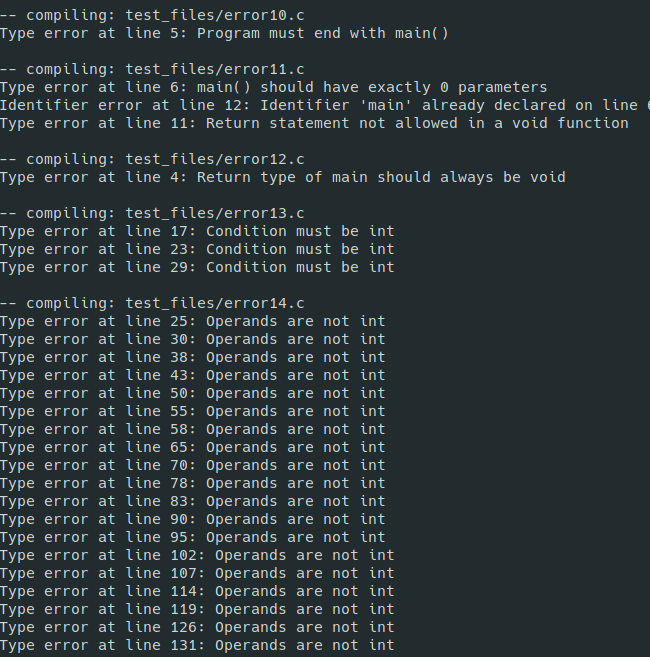
\includegraphics[scale=0.5]{figs/coverage3.png}
\caption{Semantic Analysis 의 Test Coverage.}\label{fig:coverage3}
\end{figure}

Fig.~\ref{fig:coverage3} 에서는

\begin{itemize}
\item \code{main} 함수가 소스파일의 최하단에 존재하는 여부 
\item \code{main} 함수의 인자들이 없는지 여부
\item \code{main} 함수의 리턴 타입이 void 인 여부
\item 조건문의 expression 이 int 인지 여부
\item operator 들의 operand expression 들이 int 인지 여부
\end{itemize}

등을 체크하는 것을 확인할 수 있고, 

\subsection{Symbol Table Dump}

\begin{figure}[H]
  \centering
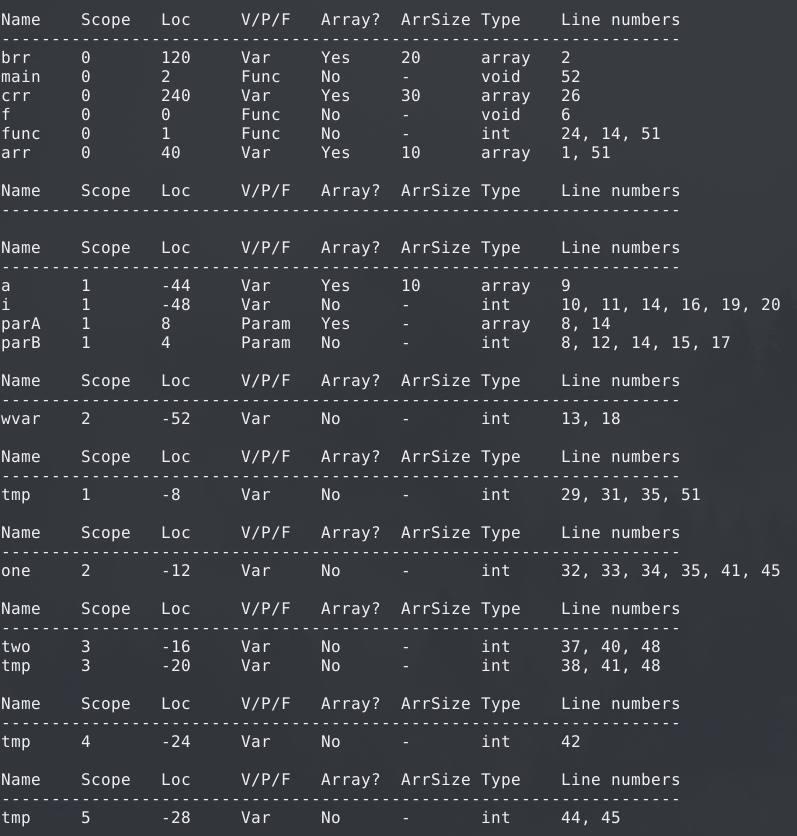
\includegraphics[scale=0.5]{figs/testresult.png}
\caption{Output}
\label{fig:output}
\end{figure}

Section.~\ref{case} 의 테스트 코드를 컴파일한 후, symbol table을 덤프한 결과는 Fig.~\ref{fig:output} 과 같다. 각 스코프 순서대로 symbol table 이 나눠서 출력되는 것을 볼 수 있다. 그리고 이 때, 각 식별자의 record 에 \textbf{scope id}, \textbf{memory location}, \textbf{식별자 종류}, \textbf{Array 여부}, \textbf{식별자 Type}, \textbf{참조되는 줄 번호} 가 출력되는 것을 볼 수 있다.


\section{기타}

\subsection{연구 조원 기여도}
\begin{itemize}
	\item 김규래: 50\%
	\item 박건: 50\%
\end{itemize}

\subsection{자체 평가}
Symbol table을 Global로 처리하지 않고, Opaque pointer \texttt{SymTable}핸들로 관리하여 메모리 누수를 방지하고 reentrancy를 보존하였다.

\subsection{느낀 점}
이번 프로젝트에서는 변수의 가능한 타입이 \texttt{int}밖에 없어서 Semantic Analysis가 간단했지만, 여러 타입이 추가되면 훨씬 어려워질 것이라는 생각이 들었다.

\end{document}
